Τα σχήματα \ref{fig:appendix:03_04:sim_orientation_position_errors}
και \ref{fig:appendix:03_04:csal_orientation_position_errors} απεικονίζουν
τα μέσα σφάλματα προσανατολισμού και στάσης των δύο μεθόδων PLICP και PGL-FMIC
που αφορούν στα πειράματα της ενότητας \ref{subsection:02_03_04:02} υπό
την πειραματική διαδικασία της ενότητας \ref{subsection:02_03_04:01}.

\begin{figure}
  \begin{subfigure}{0.5\linewidth}
    % GNUPLOT: LaTeX picture with Postscript
\begingroup
  \makeatletter
  \providecommand\color[2][]{%
    \GenericError{(gnuplot) \space\space\space\@spaces}{%
      Package color not loaded in conjunction with
      terminal option `colourtext'%
    }{See the gnuplot documentation for explanation.%
    }{Either use 'blacktext' in gnuplot or load the package
      color.sty in LaTeX.}%
    \renewcommand\color[2][]{}%
  }%
  \providecommand\includegraphics[2][]{%
    \GenericError{(gnuplot) \space\space\space\@spaces}{%
      Package graphicx or graphics not loaded%
    }{See the gnuplot documentation for explanation.%
    }{The gnuplot epslatex terminal needs graphicx.sty or graphics.sty.}%
    \renewcommand\includegraphics[2][]{}%
  }%
  \providecommand\rotatebox[2]{#2}%
  \@ifundefined{ifGPcolor}{%
    \newif\ifGPcolor
    \GPcolorfalse
  }{}%
  \@ifundefined{ifGPblacktext}{%
    \newif\ifGPblacktext
    \GPblacktexttrue
  }{}%
  % define a \g@addto@macro without @ in the name:
  \let\gplgaddtomacro\g@addto@macro
  % define empty templates for all commands taking text:
  \gdef\gplfronttext{}%
  \gdef\gplfronttext{}%
  \makeatother
  \ifGPblacktext
    % no textcolor at all
    \def\colorrgb#1{}%
    \def\colorgray#1{}%
  \else
    % gray or color?
    \ifGPcolor
      \def\colorrgb#1{\color[rgb]{#1}}%
      \def\colorgray#1{\color[gray]{#1}}%
      \expandafter\def\csname LTw\endcsname{\color{white}}%
      \expandafter\def\csname LTb\endcsname{\color{black}}%
      \expandafter\def\csname LTa\endcsname{\color{black}}%
      \expandafter\def\csname LT0\endcsname{\color[rgb]{1,0,0}}%
      \expandafter\def\csname LT1\endcsname{\color[rgb]{0,1,0}}%
      \expandafter\def\csname LT2\endcsname{\color[rgb]{0,0,1}}%
      \expandafter\def\csname LT3\endcsname{\color[rgb]{1,0,1}}%
      \expandafter\def\csname LT4\endcsname{\color[rgb]{0,1,1}}%
      \expandafter\def\csname LT5\endcsname{\color[rgb]{1,1,0}}%
      \expandafter\def\csname LT6\endcsname{\color[rgb]{0,0,0}}%
      \expandafter\def\csname LT7\endcsname{\color[rgb]{1,0.3,0}}%
      \expandafter\def\csname LT8\endcsname{\color[rgb]{0.5,0.5,0.5}}%
    \else
      % gray
      \def\colorrgb#1{\color{black}}%
      \def\colorgray#1{\color[gray]{#1}}%
      \expandafter\def\csname LTw\endcsname{\color{white}}%
      \expandafter\def\csname LTb\endcsname{\color{black}}%
      \expandafter\def\csname LTa\endcsname{\color{black}}%
      \expandafter\def\csname LT0\endcsname{\color{black}}%
      \expandafter\def\csname LT1\endcsname{\color{black}}%
      \expandafter\def\csname LT2\endcsname{\color{black}}%
      \expandafter\def\csname LT3\endcsname{\color{black}}%
      \expandafter\def\csname LT4\endcsname{\color{black}}%
      \expandafter\def\csname LT5\endcsname{\color{black}}%
      \expandafter\def\csname LT6\endcsname{\color{black}}%
      \expandafter\def\csname LT7\endcsname{\color{black}}%
      \expandafter\def\csname LT8\endcsname{\color{black}}%
    \fi
  \fi
  \setlength{\unitlength}{0.0500bp}%
  \begin{picture}(4800.00,12000.00)%
    \gplgaddtomacro\gplfronttext{%
      \colorrgb{0.00,0.00,0.00}%
      \put(492,9720){\makebox(0,0)[r]{\strut{}\small $0.0$}}%
      \colorrgb{0.00,0.00,0.00}%
      \put(492,9950){\makebox(0,0)[r]{\strut{}\small $0.002$}}%
      \colorrgb{0.00,0.00,0.00}%
      \put(492,10180){\makebox(0,0)[r]{\strut{}\small $0.004$}}%
      \colorrgb{0.00,0.00,0.00}%
      \put(492,10410){\makebox(0,0)[r]{\strut{}\small $0.006$}}%
      \colorrgb{0.00,0.00,0.00}%
      \put(492,10639){\makebox(0,0)[r]{\strut{}\small $0.008$}}%
      \colorrgb{0.00,0.00,0.00}%
      \put(492,10869){\makebox(0,0)[r]{\strut{}\small $0.010$}}%
      \colorrgb{0.00,0.00,0.00}%
      \put(492,11099){\makebox(0,0)[r]{\strut{}\small $0.012$}}%
      \colorrgb{0.00,0.00,0.00}%
      \put(874,9500){\makebox(0,0){\strut{}}}%
      \colorrgb{0.00,0.00,0.00}%
      \put(1374,9500){\makebox(0,0){\strut{}}}%
      \colorrgb{0.00,0.00,0.00}%
      \put(1873,9500){\makebox(0,0){\strut{}}}%
      \colorrgb{0.00,0.00,0.00}%
      \put(-474,10409){\rotatebox{90}{\makebox(0,0){\strut{}\small CORRIDOR}}}%
      \colorrgb{0.00,0.00,0.00}%
      \put(1373,11429){\makebox(0,0){\strut{}PLICP}}%
    }%
    \gplgaddtomacro\gplfronttext{%
    }%
    \gplgaddtomacro\gplfronttext{%
      \colorrgb{0.00,0.00,0.00}%
      \put(2712,9720){\makebox(0,0)[r]{\strut{}\small $0.0$}}%
      \colorrgb{0.00,0.00,0.00}%
      \put(2712,9950){\makebox(0,0)[r]{\strut{}\small $0.002$}}%
      \colorrgb{0.00,0.00,0.00}%
      \put(2712,10180){\makebox(0,0)[r]{\strut{}\small $0.004$}}%
      \colorrgb{0.00,0.00,0.00}%
      \put(2712,10410){\makebox(0,0)[r]{\strut{}\small $0.006$}}%
      \colorrgb{0.00,0.00,0.00}%
      \put(2712,10639){\makebox(0,0)[r]{\strut{}\small $0.008$}}%
      \colorrgb{0.00,0.00,0.00}%
      \put(2712,10869){\makebox(0,0)[r]{\strut{}\small $0.010$}}%
      \colorrgb{0.00,0.00,0.00}%
      \put(2712,11099){\makebox(0,0)[r]{\strut{}\small $0.012$}}%
      \colorrgb{0.00,0.00,0.00}%
      \put(3094,9500){\makebox(0,0){\strut{}}}%
      \colorrgb{0.00,0.00,0.00}%
      \put(3594,9500){\makebox(0,0){\strut{}}}%
      \colorrgb{0.00,0.00,0.00}%
      \put(4093,9500){\makebox(0,0){\strut{}}}%
      \colorrgb{0.00,0.00,0.00}%
      \put(3593,11429){\makebox(0,0){\strut{}PGL-FMIC}}%
    }%
    \gplgaddtomacro\gplfronttext{%
    }%
    \gplgaddtomacro\gplfronttext{%
      \colorrgb{0.00,0.00,0.00}%
      \put(492,7830){\makebox(0,0)[r]{\strut{}\small $0.0$}}%
      \colorrgb{0.00,0.00,0.00}%
      \put(492,8290){\makebox(0,0)[r]{\strut{}\small $0.005$}}%
      \colorrgb{0.00,0.00,0.00}%
      \put(492,8749){\makebox(0,0)[r]{\strut{}\small $0.01$}}%
      \colorrgb{0.00,0.00,0.00}%
      \put(492,9209){\makebox(0,0)[r]{\strut{}\small $0.015$}}%
      \colorrgb{0.00,0.00,0.00}%
      \put(874,7610){\makebox(0,0){\strut{}}}%
      \colorrgb{0.00,0.00,0.00}%
      \put(1374,7610){\makebox(0,0){\strut{}}}%
      \colorrgb{0.00,0.00,0.00}%
      \put(1873,7610){\makebox(0,0){\strut{}}}%
      \colorrgb{0.00,0.00,0.00}%
      \put(-474,8519){\rotatebox{90}{\makebox(0,0){\strut{}\small HOME}}}%
    }%
    \gplgaddtomacro\gplfronttext{%
    }%
    \gplgaddtomacro\gplfronttext{%
      \colorrgb{0.00,0.00,0.00}%
      \put(2712,7830){\makebox(0,0)[r]{\strut{}\small $0.0$}}%
      \colorrgb{0.00,0.00,0.00}%
      \put(2712,8290){\makebox(0,0)[r]{\strut{}\small $0.005$}}%
      \colorrgb{0.00,0.00,0.00}%
      \put(2712,8749){\makebox(0,0)[r]{\strut{}\small $0.01$}}%
      \colorrgb{0.00,0.00,0.00}%
      \put(2712,9209){\makebox(0,0)[r]{\strut{}\small $0.015$}}%
      \colorrgb{0.00,0.00,0.00}%
      \put(3094,7610){\makebox(0,0){\strut{}}}%
      \colorrgb{0.00,0.00,0.00}%
      \put(3594,7610){\makebox(0,0){\strut{}}}%
      \colorrgb{0.00,0.00,0.00}%
      \put(4093,7610){\makebox(0,0){\strut{}}}%
    }%
    \gplgaddtomacro\gplfronttext{%
    }%
    \gplgaddtomacro\gplfronttext{%
      \colorrgb{0.00,0.00,0.00}%
      \put(492,5940){\makebox(0,0)[r]{\strut{}\small $3.04$}}%
      \colorrgb{0.00,0.00,0.00}%
      \put(492,6170){\makebox(0,0)[r]{\strut{}\small $3.06$}}%
      \colorrgb{0.00,0.00,0.00}%
      \put(492,6400){\makebox(0,0)[r]{\strut{}\small $3.08$}}%
      \colorrgb{0.00,0.00,0.00}%
      \put(492,6630){\makebox(0,0)[r]{\strut{}\small $3.10$}}%
      \colorrgb{0.00,0.00,0.00}%
      \put(492,6859){\makebox(0,0)[r]{\strut{}\small $3.12$}}%
      \colorrgb{0.00,0.00,0.00}%
      \put(492,7089){\makebox(0,0)[r]{\strut{}\small $3.14$}}%
      \colorrgb{0.00,0.00,0.00}%
      \put(492,7319){\makebox(0,0)[r]{\strut{}\small $3.16$}}%
      \colorrgb{0.00,0.00,0.00}%
      \put(874,5720){\makebox(0,0){\strut{}}}%
      \colorrgb{0.00,0.00,0.00}%
      \put(1374,5720){\makebox(0,0){\strut{}}}%
      \colorrgb{0.00,0.00,0.00}%
      \put(1873,5720){\makebox(0,0){\strut{}}}%
      \colorrgb{0.00,0.00,0.00}%
      \put(-474,6629){\rotatebox{90}{\makebox(0,0){\strut{}\small WAREHOUSE}}}%
    }%
    \gplgaddtomacro\gplfronttext{%
    }%
    \gplgaddtomacro\gplfronttext{%
      \colorrgb{0.00,0.00,0.00}%
      \put(2712,5940){\makebox(0,0)[r]{\strut{}\small $0.0$}}%
      \colorrgb{0.00,0.00,0.00}%
      \put(2712,6285){\makebox(0,0)[r]{\strut{}\small $0.005$}}%
      \colorrgb{0.00,0.00,0.00}%
      \put(2712,6630){\makebox(0,0)[r]{\strut{}\small $0.010$}}%
      \colorrgb{0.00,0.00,0.00}%
      \put(2712,6974){\makebox(0,0)[r]{\strut{}\small $0.015$}}%
      \colorrgb{0.00,0.00,0.00}%
      \put(2712,7319){\makebox(0,0)[r]{\strut{}\small $0.020$}}%
      \colorrgb{0.00,0.00,0.00}%
      \put(3094,5720){\makebox(0,0){\strut{}}}%
      \colorrgb{0.00,0.00,0.00}%
      \put(3594,5720){\makebox(0,0){\strut{}}}%
      \colorrgb{0.00,0.00,0.00}%
      \put(4093,5720){\makebox(0,0){\strut{}}}%
    }%
    \gplgaddtomacro\gplfronttext{%
    }%
    \gplgaddtomacro\gplfronttext{%
      \colorrgb{0.00,0.00,0.00}%
      \put(492,4050){\makebox(0,0)[r]{\strut{}\small $0.0$}}%
      \colorrgb{0.00,0.00,0.00}%
      \put(492,4625){\makebox(0,0)[r]{\strut{}\small $0.50$}}%
      \colorrgb{0.00,0.00,0.00}%
      \put(492,5199){\makebox(0,0)[r]{\strut{}\small $1.0$}}%
      \colorrgb{0.00,0.00,0.00}%
      \put(492,5429){\makebox(0,0)[r]{\strut{}\small $1.2$}}%
      \colorrgb{0.00,0.00,0.00}%
      \put(874,3830){\makebox(0,0){\strut{}}}%
      \colorrgb{0.00,0.00,0.00}%
      \put(1374,3830){\makebox(0,0){\strut{}}}%
      \colorrgb{0.00,0.00,0.00}%
      \put(1873,3830){\makebox(0,0){\strut{}}}%
      \colorrgb{0.00,0.00,0.00}%
      \put(-474,4739){\rotatebox{90}{\makebox(0,0){\strut{}\small WILLOWGARAGE}}}%
    }%
    \gplgaddtomacro\gplfronttext{%
    }%
    \gplgaddtomacro\gplfronttext{%
      \colorrgb{0.00,0.00,0.00}%
      \put(2712,4050){\makebox(0,0)[r]{\strut{}\small $0.0$}}%
      \colorrgb{0.00,0.00,0.00}%
      \put(2712,4234){\makebox(0,0)[r]{\strut{}\small $0.02$}}%
      \colorrgb{0.00,0.00,0.00}%
      \put(2712,4510){\makebox(0,0)[r]{\strut{}\small $0.05$}}%
      \colorrgb{0.00,0.00,0.00}%
      \put(2712,4969){\makebox(0,0)[r]{\strut{}\small $0.10$}}%
      \colorrgb{0.00,0.00,0.00}%
      \put(2712,5429){\makebox(0,0)[r]{\strut{}\small $0.15$}}%
      \colorrgb{0.00,0.00,0.00}%
      \put(3094,3830){\makebox(0,0){\strut{}}}%
      \colorrgb{0.00,0.00,0.00}%
      \put(3594,3830){\makebox(0,0){\strut{}}}%
      \colorrgb{0.00,0.00,0.00}%
      \put(4093,3830){\makebox(0,0){\strut{}}}%
    }%
    \gplgaddtomacro\gplfronttext{%
    }%
    \gplgaddtomacro\gplfronttext{%
      \colorrgb{0.00,0.00,0.00}%
      \put(492,2160){\makebox(0,0)[r]{\strut{}\small $0.0$}}%
      \colorrgb{0.00,0.00,0.00}%
      \put(492,2436){\makebox(0,0)[r]{\strut{}\small $0.005$}}%
      \colorrgb{0.00,0.00,0.00}%
      \put(492,2712){\makebox(0,0)[r]{\strut{}\small $0.010$}}%
      \colorrgb{0.00,0.00,0.00}%
      \put(492,2987){\makebox(0,0)[r]{\strut{}\small $0.015$}}%
      \colorrgb{0.00,0.00,0.00}%
      \put(492,3263){\makebox(0,0)[r]{\strut{}\small $0.020$}}%
      \colorrgb{0.00,0.00,0.00}%
      \put(492,3539){\makebox(0,0)[r]{\strut{}\small $0.025$}}%
      \colorrgb{0.00,0.00,0.00}%
      \put(874,1940){\makebox(0,0){\strut{}\scriptsize  $0.01$}}%
      \colorrgb{0.00,0.00,0.00}%
      \put(1374,1940){\makebox(0,0){\strut{}\scriptsize  $0.02$}}%
      \colorrgb{0.00,0.00,0.00}%
      \put(1873,1940){\makebox(0,0){\strut{}\scriptsize  $0.05$}}%
      \colorrgb{0.00,0.00,0.00}%
      \put(-474,2849){\rotatebox{90}{\makebox(0,0){\strut{}\small LANDFILL}}}%
    }%
    \gplgaddtomacro\gplfronttext{%
    }%
    \gplgaddtomacro\gplfronttext{%
      \colorrgb{0.00,0.00,0.00}%
      \put(2712,2160){\makebox(0,0)[r]{\strut{}\small $0.0$}}%
      \colorrgb{0.00,0.00,0.00}%
      \put(2712,2436){\makebox(0,0)[r]{\strut{}\small $0.005$}}%
      \colorrgb{0.00,0.00,0.00}%
      \put(2712,2712){\makebox(0,0)[r]{\strut{}\small $0.010$}}%
      \colorrgb{0.00,0.00,0.00}%
      \put(2712,2987){\makebox(0,0)[r]{\strut{}\small $0.015$}}%
      \colorrgb{0.00,0.00,0.00}%
      \put(2712,3263){\makebox(0,0)[r]{\strut{}\small $0.020$}}%
      \colorrgb{0.00,0.00,0.00}%
      \put(2712,3539){\makebox(0,0)[r]{\strut{}\small $0.025$}}%
      \colorrgb{0.00,0.00,0.00}%
      \put(3094,1940){\makebox(0,0){\strut{}\scriptsize  $0.01$}}%
      \colorrgb{0.00,0.00,0.00}%
      \put(3594,1940){\makebox(0,0){\strut{}\scriptsize  $0.02$}}%
      \colorrgb{0.00,0.00,0.00}%
      \put(4093,1940){\makebox(0,0){\strut{}\scriptsize  $0.05$}}%
      \colorrgb{0.00,0.00,0.00}%
      \put(2500,1610){\makebox(0,0){\strut{}\small $d$ [m]: Θόρυβος μέτρησης $\mathcal{N}(0.0,d)$}}%
    }%
    \gplgaddtomacro\gplfronttext{%
    }%
    \put(0,0){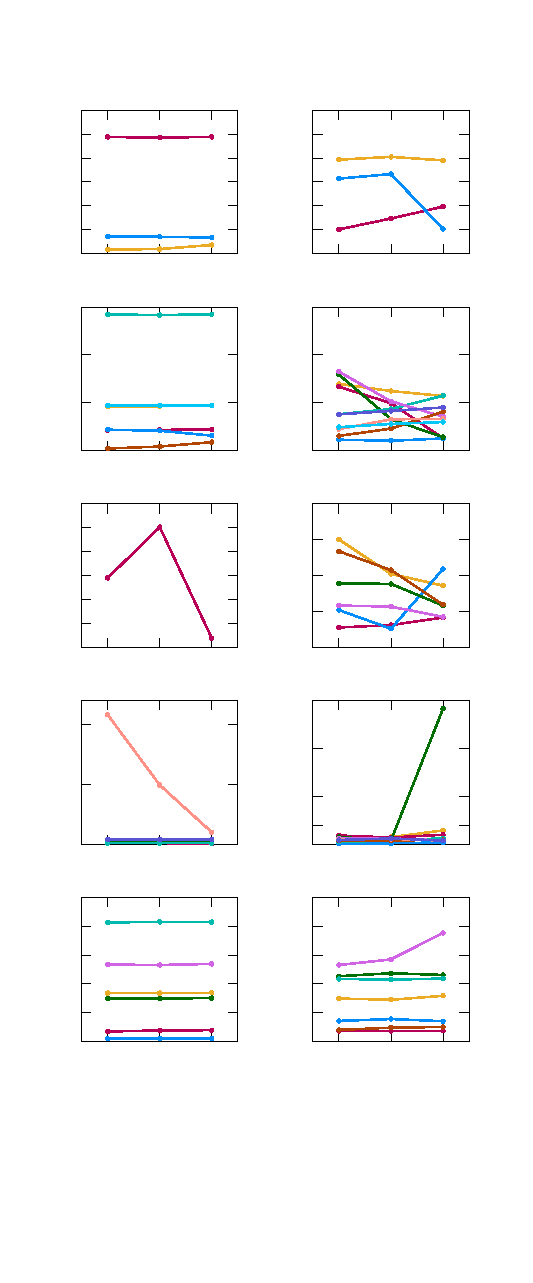
\includegraphics{./figures/parts/appendix/chapters/03/sections/04/simulations_orientation_errors}}%
    \gplfronttext
  \end{picture}%
\endgroup

  \end{subfigure}\hspace{1.0cm}
  \begin{subfigure}{0.5\linewidth}
    % GNUPLOT: LaTeX picture with Postscript
\begingroup
  \makeatletter
  \providecommand\color[2][]{%
    \GenericError{(gnuplot) \space\space\space\@spaces}{%
      Package color not loaded in conjunction with
      terminal option `colourtext'%
    }{See the gnuplot documentation for explanation.%
    }{Either use 'blacktext' in gnuplot or load the package
      color.sty in LaTeX.}%
    \renewcommand\color[2][]{}%
  }%
  \providecommand\includegraphics[2][]{%
    \GenericError{(gnuplot) \space\space\space\@spaces}{%
      Package graphicx or graphics not loaded%
    }{See the gnuplot documentation for explanation.%
    }{The gnuplot epslatex terminal needs graphicx.sty or graphics.sty.}%
    \renewcommand\includegraphics[2][]{}%
  }%
  \providecommand\rotatebox[2]{#2}%
  \@ifundefined{ifGPcolor}{%
    \newif\ifGPcolor
    \GPcolorfalse
  }{}%
  \@ifundefined{ifGPblacktext}{%
    \newif\ifGPblacktext
    \GPblacktexttrue
  }{}%
  % define a \g@addto@macro without @ in the name:
  \let\gplgaddtomacro\g@addto@macro
  % define empty templates for all commands taking text:
  \gdef\gplfronttext{}%
  \gdef\gplfronttext{}%
  \makeatother
  \ifGPblacktext
    % no textcolor at all
    \def\colorrgb#1{}%
    \def\colorgray#1{}%
  \else
    % gray or color?
    \ifGPcolor
      \def\colorrgb#1{\color[rgb]{#1}}%
      \def\colorgray#1{\color[gray]{#1}}%
      \expandafter\def\csname LTw\endcsname{\color{white}}%
      \expandafter\def\csname LTb\endcsname{\color{black}}%
      \expandafter\def\csname LTa\endcsname{\color{black}}%
      \expandafter\def\csname LT0\endcsname{\color[rgb]{1,0,0}}%
      \expandafter\def\csname LT1\endcsname{\color[rgb]{0,1,0}}%
      \expandafter\def\csname LT2\endcsname{\color[rgb]{0,0,1}}%
      \expandafter\def\csname LT3\endcsname{\color[rgb]{1,0,1}}%
      \expandafter\def\csname LT4\endcsname{\color[rgb]{0,1,1}}%
      \expandafter\def\csname LT5\endcsname{\color[rgb]{1,1,0}}%
      \expandafter\def\csname LT6\endcsname{\color[rgb]{0,0,0}}%
      \expandafter\def\csname LT7\endcsname{\color[rgb]{1,0.3,0}}%
      \expandafter\def\csname LT8\endcsname{\color[rgb]{0.5,0.5,0.5}}%
    \else
      % gray
      \def\colorrgb#1{\color{black}}%
      \def\colorgray#1{\color[gray]{#1}}%
      \expandafter\def\csname LTw\endcsname{\color{white}}%
      \expandafter\def\csname LTb\endcsname{\color{black}}%
      \expandafter\def\csname LTa\endcsname{\color{black}}%
      \expandafter\def\csname LT0\endcsname{\color{black}}%
      \expandafter\def\csname LT1\endcsname{\color{black}}%
      \expandafter\def\csname LT2\endcsname{\color{black}}%
      \expandafter\def\csname LT3\endcsname{\color{black}}%
      \expandafter\def\csname LT4\endcsname{\color{black}}%
      \expandafter\def\csname LT5\endcsname{\color{black}}%
      \expandafter\def\csname LT6\endcsname{\color{black}}%
      \expandafter\def\csname LT7\endcsname{\color{black}}%
      \expandafter\def\csname LT8\endcsname{\color{black}}%
    \fi
  \fi
  \setlength{\unitlength}{0.0500bp}%
  \begin{picture}(4800.00,12000.00)%
    \gplgaddtomacro\gplfronttext{%
      \colorrgb{0.00,0.00,0.00}%
      \put(492,9720){\makebox(0,0)[r]{\strut{}\small $0.0$}}%
      \colorrgb{0.00,0.00,0.00}%
      \put(492,9996){\makebox(0,0)[r]{\strut{}\small $0.01$}}%
      \colorrgb{0.00,0.00,0.00}%
      \put(492,10272){\makebox(0,0)[r]{\strut{}\small $0.02$}}%
      \colorrgb{0.00,0.00,0.00}%
      \put(492,10547){\makebox(0,0)[r]{\strut{}\small $0.03$}}%
      \colorrgb{0.00,0.00,0.00}%
      \put(492,10823){\makebox(0,0)[r]{\strut{}\small $0.04$}}%
      \colorrgb{0.00,0.00,0.00}%
      \put(492,11099){\makebox(0,0)[r]{\strut{}\small $0.05$}}%
      \colorrgb{0.00,0.00,0.00}%
      \put(874,9500){\makebox(0,0){\strut{}}}%
      \colorrgb{0.00,0.00,0.00}%
      \put(1374,9500){\makebox(0,0){\strut{}}}%
      \colorrgb{0.00,0.00,0.00}%
      \put(1873,9500){\makebox(0,0){\strut{}}}%
      \colorrgb{0.00,0.00,0.00}%
      %\put(-542,10409){\rotatebox{90}{\makebox(0,0){\strut{}\small CORRIDOR}}}%
      \colorrgb{0.00,0.00,0.00}%
      \put(1373,11429){\makebox(0,0){\strut{}PLICP}}%
    }%
    \gplgaddtomacro\gplfronttext{%
    }%
    \gplgaddtomacro\gplfronttext{%
      \colorrgb{0.00,0.00,0.00}%
      \put(2712,9720){\makebox(0,0)[r]{\strut{}\small $0.0$}}%
      \colorrgb{0.00,0.00,0.00}%
      \put(2712,9996){\makebox(0,0)[r]{\strut{}\small $0.01$}}%
      \colorrgb{0.00,0.00,0.00}%
      \put(2712,10272){\makebox(0,0)[r]{\strut{}\small $0.02$}}%
      \colorrgb{0.00,0.00,0.00}%
      \put(2712,10547){\makebox(0,0)[r]{\strut{}\small $0.03$}}%
      \colorrgb{0.00,0.00,0.00}%
      \put(2712,10823){\makebox(0,0)[r]{\strut{}\small $0.04$}}%
      \colorrgb{0.00,0.00,0.00}%
      \put(2712,11099){\makebox(0,0)[r]{\strut{}\small $0.05$}}%
      \colorrgb{0.00,0.00,0.00}%
      \put(3094,9500){\makebox(0,0){\strut{}}}%
      \colorrgb{0.00,0.00,0.00}%
      \put(3594,9500){\makebox(0,0){\strut{}}}%
      \colorrgb{0.00,0.00,0.00}%
      \put(4093,9500){\makebox(0,0){\strut{}}}%
      \colorrgb{0.00,0.00,0.00}%
      \put(3593,11429){\makebox(0,0){\strut{}PGL-FMIC}}%
    }%
    \gplgaddtomacro\gplfronttext{%
    }%
    \gplgaddtomacro\gplfronttext{%
      \colorrgb{0.00,0.00,0.00}%
      \put(492,7830){\makebox(0,0)[r]{\strut{}\small $0.0$}}%
      \colorrgb{0.00,0.00,0.00}%
      \put(492,8106){\makebox(0,0)[r]{\strut{}\small $0.05$}}%
      \colorrgb{0.00,0.00,0.00}%
      \put(492,8382){\makebox(0,0)[r]{\strut{}\small $0.10$}}%
      \colorrgb{0.00,0.00,0.00}%
      \put(492,8657){\makebox(0,0)[r]{\strut{}\small $0.15$}}%
      \colorrgb{0.00,0.00,0.00}%
      \put(492,8933){\makebox(0,0)[r]{\strut{}\small $0.20$}}%
      \colorrgb{0.00,0.00,0.00}%
      \put(492,9209){\makebox(0,0)[r]{\strut{}\small $0.25$}}%
      \colorrgb{0.00,0.00,0.00}%
      \put(874,7610){\makebox(0,0){\strut{}}}%
      \colorrgb{0.00,0.00,0.00}%
      \put(1374,7610){\makebox(0,0){\strut{}}}%
      \colorrgb{0.00,0.00,0.00}%
      \put(1873,7610){\makebox(0,0){\strut{}}}%
      \colorrgb{0.00,0.00,0.00}%
      %\put(-542,8519){\rotatebox{90}{\makebox(0,0){\strut{}\small HOME}}}%
    }%
    \gplgaddtomacro\gplfronttext{%
    }%
    \gplgaddtomacro\gplfronttext{%
      \colorrgb{0.00,0.00,0.00}%
      \put(2712,7830){\makebox(0,0)[r]{\strut{}\small $0.0$}}%
      \colorrgb{0.00,0.00,0.00}%
      \put(2712,8106){\makebox(0,0)[r]{\strut{}\small $0.05$}}%
      \colorrgb{0.00,0.00,0.00}%
      \put(2712,8382){\makebox(0,0)[r]{\strut{}\small $0.10$}}%
      \colorrgb{0.00,0.00,0.00}%
      \put(2712,8657){\makebox(0,0)[r]{\strut{}\small $0.15$}}%
      \colorrgb{0.00,0.00,0.00}%
      \put(2712,8933){\makebox(0,0)[r]{\strut{}\small $0.20$}}%
      \colorrgb{0.00,0.00,0.00}%
      \put(2712,9209){\makebox(0,0)[r]{\strut{}\small $0.25$}}%
      \colorrgb{0.00,0.00,0.00}%
      \put(3094,7610){\makebox(0,0){\strut{}}}%
      \colorrgb{0.00,0.00,0.00}%
      \put(3594,7610){\makebox(0,0){\strut{}}}%
      \colorrgb{0.00,0.00,0.00}%
      \put(4093,7610){\makebox(0,0){\strut{}}}%
    }%
    \gplgaddtomacro\gplfronttext{%
    }%
    \gplgaddtomacro\gplfronttext{%
      \colorrgb{0.00,0.00,0.00}%
      \put(492,5940){\makebox(0,0)[r]{\strut{}\small $0.785$}}%
      \colorrgb{0.00,0.00,0.00}%
      \put(492,6216){\makebox(0,0)[r]{\strut{}\small $0.790$}}%
      \colorrgb{0.00,0.00,0.00}%
      \put(492,6492){\makebox(0,0)[r]{\strut{}\small $0.795$}}%
      \colorrgb{0.00,0.00,0.00}%
      \put(492,6767){\makebox(0,0)[r]{\strut{}\small $0.800$}}%
      \colorrgb{0.00,0.00,0.00}%
      \put(492,7043){\makebox(0,0)[r]{\strut{}\small $0.805$}}%
      \colorrgb{0.00,0.00,0.00}%
      \put(492,7319){\makebox(0,0)[r]{\strut{}\small $0.810$}}%
      \colorrgb{0.00,0.00,0.00}%
      \put(811,5720){\makebox(0,0){\strut{}}}%
      \colorrgb{0.00,0.00,0.00}%
      \put(1186,5720){\makebox(0,0){\strut{}}}%
      \colorrgb{0.00,0.00,0.00}%
      \put(1561,5720){\makebox(0,0){\strut{}}}%
      \colorrgb{0.00,0.00,0.00}%
      %\put(-674,6629){\rotatebox{90}{\makebox(0,0){\strut{}\small WAREHOUSE}}}%
    }%
    \gplgaddtomacro\gplfronttext{%
    }%
    \gplgaddtomacro\gplfronttext{%
      \colorrgb{0.00,0.00,0.00}%
      \put(2712,5940){\makebox(0,0)[r]{\strut{}\small $0.0$}}%
      \colorrgb{0.00,0.00,0.00}%
      \put(2712,6216){\makebox(0,0)[r]{\strut{}\small $0.03$}}%
      \colorrgb{0.00,0.00,0.00}%
      \put(2712,6400){\makebox(0,0)[r]{\strut{}\small $0.05$}}%
      \colorrgb{0.00,0.00,0.00}%
      \put(2712,6584){\makebox(0,0)[r]{\strut{}\small $0.07$}}%
      \colorrgb{0.00,0.00,0.00}%
      \put(2712,6767){\makebox(0,0)[r]{\strut{}\small $0.09$}}%
      \colorrgb{0.00,0.00,0.00}%
      \put(2712,6951){\makebox(0,0)[r]{\strut{}\small $0.11$}}%
      \colorrgb{0.00,0.00,0.00}%
      \put(2712,7135){\makebox(0,0)[r]{\strut{}\small $0.13$}}%
      \colorrgb{0.00,0.00,0.00}%
      \put(2712,7319){\makebox(0,0)[r]{\strut{}\small $0.15$}}%
      \colorrgb{0.00,0.00,0.00}%
      \put(3094,5720){\makebox(0,0){\strut{}}}%
      \colorrgb{0.00,0.00,0.00}%
      \put(3594,5720){\makebox(0,0){\strut{}}}%
      \colorrgb{0.00,0.00,0.00}%
      \put(4093,5720){\makebox(0,0){\strut{}}}%
    }%
    \gplgaddtomacro\gplfronttext{%
    }%
    \gplgaddtomacro\gplfronttext{%
      \colorrgb{0.00,0.00,0.00}%
      \put(492,4050){\makebox(0,0)[r]{\strut{}\small $0.0$}}%
      \colorrgb{0.00,0.00,0.00}%
      \put(492,4356){\makebox(0,0)[r]{\strut{}\small $0.10$}}%
      \colorrgb{0.00,0.00,0.00}%
      \put(492,4663){\makebox(0,0)[r]{\strut{}\small $0.20$}}%
      \colorrgb{0.00,0.00,0.00}%
      \put(492,4969){\makebox(0,0)[r]{\strut{}\small $0.30$}}%
      \colorrgb{0.00,0.00,0.00}%
      \put(492,5276){\makebox(0,0)[r]{\strut{}\small $0.40$}}%
      \colorrgb{0.00,0.00,0.00}%
      \put(874,3830){\makebox(0,0){\strut{}}}%
      \colorrgb{0.00,0.00,0.00}%
      \put(1374,3830){\makebox(0,0){\strut{}}}%
      \colorrgb{0.00,0.00,0.00}%
      \put(1873,3830){\makebox(0,0){\strut{}}}%
      \colorrgb{0.00,0.00,0.00}%
      %\put(-542,4739){\rotatebox{90}{\makebox(0,0){\strut{}\small WILLOWGARAGE}}}%
    }%
    \gplgaddtomacro\gplfronttext{%
    }%
    \gplgaddtomacro\gplfronttext{%
      \colorrgb{0.00,0.00,0.00}%
      \put(2712,4050){\makebox(0,0)[r]{\strut{}\small $0.0$}}%
      \colorrgb{0.00,0.00,0.00}%
      \put(2712,4356){\makebox(0,0)[r]{\strut{}\small $0.10$}}%
      \colorrgb{0.00,0.00,0.00}%
      \put(2712,4663){\makebox(0,0)[r]{\strut{}\small $0.20$}}%
      \colorrgb{0.00,0.00,0.00}%
      \put(2712,4969){\makebox(0,0)[r]{\strut{}\small $0.30$}}%
      \colorrgb{0.00,0.00,0.00}%
      \put(2712,5276){\makebox(0,0)[r]{\strut{}\small $0.40$}}%
      \colorrgb{0.00,0.00,0.00}%
      \put(3094,3830){\makebox(0,0){\strut{}}}%
      \colorrgb{0.00,0.00,0.00}%
      \put(3594,3830){\makebox(0,0){\strut{}}}%
      \colorrgb{0.00,0.00,0.00}%
      \put(4093,3830){\makebox(0,0){\strut{}}}%
    }%
    \gplgaddtomacro\gplfronttext{%
    }%
    \gplgaddtomacro\gplfronttext{%
      \colorrgb{0.00,0.00,0.00}%
      \put(492,2160){\makebox(0,0)[r]{\strut{}\small $0.25$}}%
      \colorrgb{0.00,0.00,0.00}%
      \put(492,2505){\makebox(0,0)[r]{\strut{}\small $0.30$}}%
      \colorrgb{0.00,0.00,0.00}%
      \put(492,2850){\makebox(0,0)[r]{\strut{}\small $0.35$}}%
      \colorrgb{0.00,0.00,0.00}%
      \put(492,3194){\makebox(0,0)[r]{\strut{}\small $0.40$}}%
      \colorrgb{0.00,0.00,0.00}%
      \put(492,3539){\makebox(0,0)[r]{\strut{}\small $0.45$}}%
      \colorrgb{0.00,0.00,0.00}%
      \put(874,1940){\makebox(0,0){\strut{}\scriptsize  $0.01$}}%
      \colorrgb{0.00,0.00,0.00}%
      \put(1374,1940){\makebox(0,0){\strut{}\scriptsize  $0.02$}}%
      \colorrgb{0.00,0.00,0.00}%
      \put(1873,1940){\makebox(0,0){\strut{}\scriptsize  $0.05$}}%
      \colorrgb{0.00,0.00,0.00}%
      %\put(-542,2849){\rotatebox{90}{\makebox(0,0){\strut{}\small LANDFILL}}}%
    }%
    \gplgaddtomacro\gplfronttext{%
    }%
    \gplgaddtomacro\gplfronttext{%
      \colorrgb{0.00,0.00,0.00}%
      \put(2712,2160){\makebox(0,0)[r]{\strut{}\small $0.25$}}%
      \colorrgb{0.00,0.00,0.00}%
      \put(2712,2505){\makebox(0,0)[r]{\strut{}\small $0.30$}}%
      \colorrgb{0.00,0.00,0.00}%
      \put(2712,2850){\makebox(0,0)[r]{\strut{}\small $0.35$}}%
      \colorrgb{0.00,0.00,0.00}%
      \put(2712,3194){\makebox(0,0)[r]{\strut{}\small $0.40$}}%
      \colorrgb{0.00,0.00,0.00}%
      \put(2712,3539){\makebox(0,0)[r]{\strut{}\small $0.45$}}%
      \colorrgb{0.00,0.00,0.00}%
      \put(3094,1940){\makebox(0,0){\strut{}\scriptsize  $0.01$}}%
      \colorrgb{0.00,0.00,0.00}%
      \put(3594,1940){\makebox(0,0){\strut{}\scriptsize  $0.02$}}%
      \colorrgb{0.00,0.00,0.00}%
      \put(4093,1940){\makebox(0,0){\strut{}\scriptsize  $0.05$}}%
      \colorrgb{0.00,0.00,0.00}%
      \put(2500,1610){\makebox(0,0){\strut{}\small $d$ [m]: Θόρυβος μέτρησης $\mathcal{N}(0.0,d)$}}%
    }%
    \gplgaddtomacro\gplfronttext{%
    }%
    \put(0,0){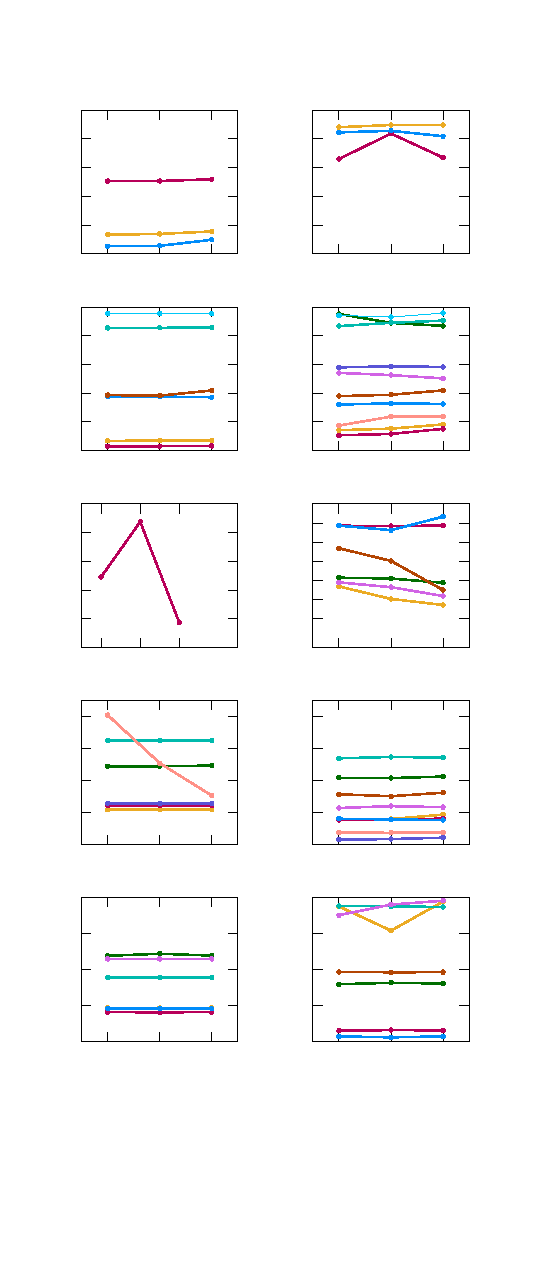
\includegraphics{./figures/parts/appendix/chapters/03/sections/04/simulations_location_errors}}%
    \gplfronttext
  \end{picture}%
\endgroup

  \end{subfigure}
  \vspace{-2.5cm}
\caption{\small Μέση τιμή σφάλματος προσανατολισμού ορθών λύσεων (αριστερά) και
         θέσης (δεξιά) ανά περιβάλλον προσομοίωσης, στάση, και τυπική απόκλιση
         θορύβου μέτρησης}
\label{fig:appendix:03_04:sim_orientation_position_errors}
\end{figure}

\begin{figure}[]
  \begin{subfigure}{0.5\linewidth}
    % GNUPLOT: LaTeX picture with Postscript
\begingroup
  \makeatletter
  \providecommand\color[2][]{%
    \GenericError{(gnuplot) \space\space\space\@spaces}{%
      Package color not loaded in conjunction with
      terminal option `colourtext'%
    }{See the gnuplot documentation for explanation.%
    }{Either use 'blacktext' in gnuplot or load the package
      color.sty in LaTeX.}%
    \renewcommand\color[2][]{}%
  }%
  \providecommand\includegraphics[2][]{%
    \GenericError{(gnuplot) \space\space\space\@spaces}{%
      Package graphicx or graphics not loaded%
    }{See the gnuplot documentation for explanation.%
    }{The gnuplot epslatex terminal needs graphicx.sty or graphics.sty.}%
    \renewcommand\includegraphics[2][]{}%
  }%
  \providecommand\rotatebox[2]{#2}%
  \@ifundefined{ifGPcolor}{%
    \newif\ifGPcolor
    \GPcolorfalse
  }{}%
  \@ifundefined{ifGPblacktext}{%
    \newif\ifGPblacktext
    \GPblacktexttrue
  }{}%
  % define a \g@addto@macro without @ in the name:
  \let\gplgaddtomacro\g@addto@macro
  % define empty templates for all commands taking text:
  \gdef\gplfronttext{}%
  \gdef\gplfronttext{}%
  \makeatother
  \ifGPblacktext
    % no textcolor at all
    \def\colorrgb#1{}%
    \def\colorgray#1{}%
  \else
    % gray or color?
    \ifGPcolor
      \def\colorrgb#1{\color[rgb]{#1}}%
      \def\colorgray#1{\color[gray]{#1}}%
      \expandafter\def\csname LTw\endcsname{\color{white}}%
      \expandafter\def\csname LTb\endcsname{\color{black}}%
      \expandafter\def\csname LTa\endcsname{\color{black}}%
      \expandafter\def\csname LT0\endcsname{\color[rgb]{1,0,0}}%
      \expandafter\def\csname LT1\endcsname{\color[rgb]{0,1,0}}%
      \expandafter\def\csname LT2\endcsname{\color[rgb]{0,0,1}}%
      \expandafter\def\csname LT3\endcsname{\color[rgb]{1,0,1}}%
      \expandafter\def\csname LT4\endcsname{\color[rgb]{0,1,1}}%
      \expandafter\def\csname LT5\endcsname{\color[rgb]{1,1,0}}%
      \expandafter\def\csname LT6\endcsname{\color[rgb]{0,0,0}}%
      \expandafter\def\csname LT7\endcsname{\color[rgb]{1,0.3,0}}%
      \expandafter\def\csname LT8\endcsname{\color[rgb]{0.5,0.5,0.5}}%
    \else
      % gray
      \def\colorrgb#1{\color{black}}%
      \def\colorgray#1{\color[gray]{#1}}%
      \expandafter\def\csname LTw\endcsname{\color{white}}%
      \expandafter\def\csname LTb\endcsname{\color{black}}%
      \expandafter\def\csname LTa\endcsname{\color{black}}%
      \expandafter\def\csname LT0\endcsname{\color{black}}%
      \expandafter\def\csname LT1\endcsname{\color{black}}%
      \expandafter\def\csname LT2\endcsname{\color{black}}%
      \expandafter\def\csname LT3\endcsname{\color{black}}%
      \expandafter\def\csname LT4\endcsname{\color{black}}%
      \expandafter\def\csname LT5\endcsname{\color{black}}%
      \expandafter\def\csname LT6\endcsname{\color{black}}%
      \expandafter\def\csname LT7\endcsname{\color{black}}%
      \expandafter\def\csname LT8\endcsname{\color{black}}%
    \fi
  \fi
  \setlength{\unitlength}{0.0500bp}%
  \begin{picture}(4000.00,3000.00)%
    \gplgaddtomacro\gplfronttext{%
      \colorrgb{0.00,0.00,0.00}%
      \put(388,1822){\makebox(0,0)[r]{\strut{}\small $0.0$}}%
      \colorrgb{0.00,0.00,0.00}%
      \put(388,2139){\makebox(0,0)[r]{\strut{}\small $0.04$}}%
      \colorrgb{0.00,0.00,0.00}%
      \put(388,2457){\makebox(0,0)[r]{\strut{}\small $0.08$}}%
      \colorrgb{0.00,0.00,0.00}%
      \put(388,2774){\makebox(0,0)[r]{\strut{}\small $0.12$}}%
      \colorrgb{0.00,0.00,0.00}%
      \put(778,1602){\makebox(0,0){\strut{}}}%
      \colorrgb{0.00,0.00,0.00}%
      \put(1037,1602){\makebox(0,0){\strut{}}}%
      \colorrgb{0.00,0.00,0.00}%
      \put(1295,1602){\makebox(0,0){\strut{}}}%
      \colorrgb{0.00,0.00,0.00}%
      \put(1553,1602){\makebox(0,0){\strut{}}}%
      \colorrgb{0.00,0.00,0.00}%
      \put(1811,1602){\makebox(0,0){\strut{}}}%
      \colorrgb{0.00,0.00,0.00}%
      \put(2070,1602){\makebox(0,0){\strut{}}}%
      \colorrgb{0.00,0.00,0.00}%
      \put(2328,1602){\makebox(0,0){\strut{}}}%
      \colorrgb{0.00,0.00,0.00}%
      \put(2586,1602){\makebox(0,0){\strut{}}}%
      \colorrgb{0.00,0.00,0.00}%
      \put(2844,1602){\makebox(0,0){\strut{}}}%
      \colorrgb{0.00,0.00,0.00}%
      \put(3103,1602){\makebox(0,0){\strut{}}}%
      \colorrgb{0.00,0.00,0.00}%
      \put(3361,1602){\makebox(0,0){\strut{}}}%
      \colorrgb{0.00,0.00,0.00}%
      \put(-446,2298){\rotatebox{90}{\makebox(0,0){\strut{}PLICP}}}%
      \colorrgb{0.00,0.00,0.00}%
      \put(2069,3104){\makebox(0,0){\strut{}Mean inlier orientation error [rad]}}%
    }%
    \gplgaddtomacro\gplfronttext{%
    }%
    \gplgaddtomacro\gplfronttext{%
      \colorrgb{0.00,0.00,0.00}%
      \put(388,330){\makebox(0,0)[r]{\strut{}\small $0.0$}}%
      \colorrgb{0.00,0.00,0.00}%
      \put(388,647){\makebox(0,0)[r]{\strut{}\small $0.04$}}%
      \colorrgb{0.00,0.00,0.00}%
      \put(388,965){\makebox(0,0)[r]{\strut{}\small $0.08$}}%
      \colorrgb{0.00,0.00,0.00}%
      \put(388,1282){\makebox(0,0)[r]{\strut{}\small $0.12$}}%
      \colorrgb{0.00,0.00,0.00}%
      \put(778,110){\makebox(0,0){\strut{}\small $\bm{p}_a^A$}}%
      \colorrgb{0.00,0.00,0.00}%
      \put(1037,110){\makebox(0,0){\strut{}\small $\bm{p}_b^A$}}%
      \colorrgb{0.00,0.00,0.00}%
      \put(1295,110){\makebox(0,0){\strut{}\small $\bm{p}_c^A$}}%
      \colorrgb{0.00,0.00,0.00}%
      \put(1553,110){\makebox(0,0){\strut{}\small $\bm{p}_d^A$}}%
      \colorrgb{0.00,0.00,0.00}%
      \put(1811,110){\makebox(0,0){\strut{}\small $\bm{p}_e^A$}}%
      \colorrgb{0.00,0.00,0.00}%
      \put(2070,110){\makebox(0,0){\strut{}\small $\bm{p}_f^A$}}%
      \colorrgb{0.00,0.00,0.00}%
      \put(2328,110){\makebox(0,0){\strut{}\small $\bm{p}_g^A$}}%
      \colorrgb{0.00,0.00,0.00}%
      \put(2586,110){\makebox(0,0){\strut{}\small $\bm{p}_h^A$}}%
      \colorrgb{0.00,0.00,0.00}%
      \put(2844,110){\makebox(0,0){\strut{}\small $\bm{p}_i^A$}}%
      \colorrgb{0.00,0.00,0.00}%
      \put(3103,110){\makebox(0,0){\strut{}\small $\bm{p}_j^A$}}%
      \colorrgb{0.00,0.00,0.00}%
      \put(3361,110){\makebox(0,0){\strut{}\small $\bm{p}_k^A$}}%
      \colorrgb{0.00,0.00,0.00}%
      \put(-446,806){\rotatebox{90}{\makebox(0,0){\strut{}PGL-FMIC}}}%
      \colorrgb{0.00,0.00,0.00}%
      \put(2069,-220){\makebox(0,0){\strut{}Σημαίνον στάσης}}%
    }%
    \gplgaddtomacro\gplfronttext{%
    }%
    \put(0,0){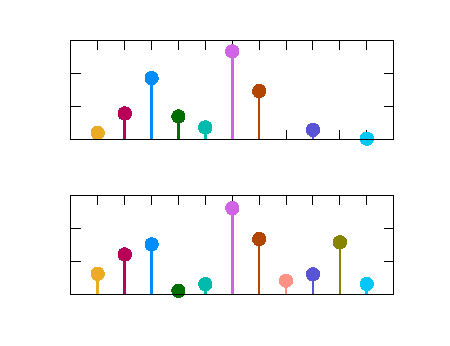
\includegraphics{./figures/parts/appendix/chapters/03/sections/04/csal_orientation_errors}}%
    \gplfronttext
  \end{picture}%
\endgroup

  \end{subfigure}\hspace{1.0cm}
  \begin{subfigure}{0.5\linewidth}
    % GNUPLOT: LaTeX picture with Postscript
\begingroup
  \makeatletter
  \providecommand\color[2][]{%
    \GenericError{(gnuplot) \space\space\space\@spaces}{%
      Package color not loaded in conjunction with
      terminal option `colourtext'%
    }{See the gnuplot documentation for explanation.%
    }{Either use 'blacktext' in gnuplot or load the package
      color.sty in LaTeX.}%
    \renewcommand\color[2][]{}%
  }%
  \providecommand\includegraphics[2][]{%
    \GenericError{(gnuplot) \space\space\space\@spaces}{%
      Package graphicx or graphics not loaded%
    }{See the gnuplot documentation for explanation.%
    }{The gnuplot epslatex terminal needs graphicx.sty or graphics.sty.}%
    \renewcommand\includegraphics[2][]{}%
  }%
  \providecommand\rotatebox[2]{#2}%
  \@ifundefined{ifGPcolor}{%
    \newif\ifGPcolor
    \GPcolorfalse
  }{}%
  \@ifundefined{ifGPblacktext}{%
    \newif\ifGPblacktext
    \GPblacktexttrue
  }{}%
  % define a \g@addto@macro without @ in the name:
  \let\gplgaddtomacro\g@addto@macro
  % define empty templates for all commands taking text:
  \gdef\gplfronttext{}%
  \gdef\gplfronttext{}%
  \makeatother
  \ifGPblacktext
    % no textcolor at all
    \def\colorrgb#1{}%
    \def\colorgray#1{}%
  \else
    % gray or color?
    \ifGPcolor
      \def\colorrgb#1{\color[rgb]{#1}}%
      \def\colorgray#1{\color[gray]{#1}}%
      \expandafter\def\csname LTw\endcsname{\color{white}}%
      \expandafter\def\csname LTb\endcsname{\color{black}}%
      \expandafter\def\csname LTa\endcsname{\color{black}}%
      \expandafter\def\csname LT0\endcsname{\color[rgb]{1,0,0}}%
      \expandafter\def\csname LT1\endcsname{\color[rgb]{0,1,0}}%
      \expandafter\def\csname LT2\endcsname{\color[rgb]{0,0,1}}%
      \expandafter\def\csname LT3\endcsname{\color[rgb]{1,0,1}}%
      \expandafter\def\csname LT4\endcsname{\color[rgb]{0,1,1}}%
      \expandafter\def\csname LT5\endcsname{\color[rgb]{1,1,0}}%
      \expandafter\def\csname LT6\endcsname{\color[rgb]{0,0,0}}%
      \expandafter\def\csname LT7\endcsname{\color[rgb]{1,0.3,0}}%
      \expandafter\def\csname LT8\endcsname{\color[rgb]{0.5,0.5,0.5}}%
    \else
      % gray
      \def\colorrgb#1{\color{black}}%
      \def\colorgray#1{\color[gray]{#1}}%
      \expandafter\def\csname LTw\endcsname{\color{white}}%
      \expandafter\def\csname LTb\endcsname{\color{black}}%
      \expandafter\def\csname LTa\endcsname{\color{black}}%
      \expandafter\def\csname LT0\endcsname{\color{black}}%
      \expandafter\def\csname LT1\endcsname{\color{black}}%
      \expandafter\def\csname LT2\endcsname{\color{black}}%
      \expandafter\def\csname LT3\endcsname{\color{black}}%
      \expandafter\def\csname LT4\endcsname{\color{black}}%
      \expandafter\def\csname LT5\endcsname{\color{black}}%
      \expandafter\def\csname LT6\endcsname{\color{black}}%
      \expandafter\def\csname LT7\endcsname{\color{black}}%
      \expandafter\def\csname LT8\endcsname{\color{black}}%
    \fi
  \fi
  \setlength{\unitlength}{0.0500bp}%
  \begin{picture}(4000.00,3000.00)%
    \gplgaddtomacro\gplfronttext{%
      \colorrgb{0.00,0.00,0.00}%
      \put(388,1822){\makebox(0,0)[r]{\strut{}\small $0.0$}}%
      \colorrgb{0.00,0.00,0.00}%
      \put(388,2094){\makebox(0,0)[r]{\strut{}\small $0.10$}}%
      \colorrgb{0.00,0.00,0.00}%
      \put(388,2366){\makebox(0,0)[r]{\strut{}\small $0.20$}}%
      \colorrgb{0.00,0.00,0.00}%
      \put(388,2638){\makebox(0,0)[r]{\strut{}\small $0.30$}}%
      \colorrgb{0.00,0.00,0.00}%
      \put(778,1602){\makebox(0,0){\strut{}}}%
      \colorrgb{0.00,0.00,0.00}%
      \put(1037,1602){\makebox(0,0){\strut{}}}%
      \colorrgb{0.00,0.00,0.00}%
      \put(1295,1602){\makebox(0,0){\strut{}}}%
      \colorrgb{0.00,0.00,0.00}%
      \put(1553,1602){\makebox(0,0){\strut{}}}%
      \colorrgb{0.00,0.00,0.00}%
      \put(1811,1602){\makebox(0,0){\strut{}}}%
      \colorrgb{0.00,0.00,0.00}%
      \put(2070,1602){\makebox(0,0){\strut{}}}%
      \colorrgb{0.00,0.00,0.00}%
      \put(2328,1602){\makebox(0,0){\strut{}}}%
      \colorrgb{0.00,0.00,0.00}%
      \put(2586,1602){\makebox(0,0){\strut{}}}%
      \colorrgb{0.00,0.00,0.00}%
      \put(2844,1602){\makebox(0,0){\strut{}}}%
      \colorrgb{0.00,0.00,0.00}%
      \put(3103,1602){\makebox(0,0){\strut{}}}%
      \colorrgb{0.00,0.00,0.00}%
      \put(3361,1602){\makebox(0,0){\strut{}}}%
      \colorrgb{0.00,0.00,0.00}%
      %\put(-646,2298){\rotatebox{90}{\makebox(0,0){\strut{}PLICP}}}%
      \colorrgb{0.00,0.00,0.00}%
      \put(2069,3104){\makebox(0,0){\strut{}Mean inlier location error [m]}}%
    }%
    \gplgaddtomacro\gplfronttext{%
    }%
    \gplgaddtomacro\gplfronttext{%
      \colorrgb{0.00,0.00,0.00}%
      \put(388,330){\makebox(0,0)[r]{\strut{}\small $0.0$}}%
      \colorrgb{0.00,0.00,0.00}%
      \put(388,602){\makebox(0,0)[r]{\strut{}\small $0.10$}}%
      \colorrgb{0.00,0.00,0.00}%
      \put(388,874){\makebox(0,0)[r]{\strut{}\small $0.20$}}%
      \colorrgb{0.00,0.00,0.00}%
      \put(388,1146){\makebox(0,0)[r]{\strut{}\small $0.30$}}%
      \colorrgb{0.00,0.00,0.00}%
      \put(778,110){\makebox(0,0){\strut{}\small $\bm{p}_a^A$}}%
      \colorrgb{0.00,0.00,0.00}%
      \put(1037,110){\makebox(0,0){\strut{}\small $\bm{p}_b^A$}}%
      \colorrgb{0.00,0.00,0.00}%
      \put(1295,110){\makebox(0,0){\strut{}\small $\bm{p}_c^A$}}%
      \colorrgb{0.00,0.00,0.00}%
      \put(1553,110){\makebox(0,0){\strut{}\small $\bm{p}_d^A$}}%
      \colorrgb{0.00,0.00,0.00}%
      \put(1811,110){\makebox(0,0){\strut{}\small $\bm{p}_e^A$}}%
      \colorrgb{0.00,0.00,0.00}%
      \put(2070,110){\makebox(0,0){\strut{}\small $\bm{p}_f^A$}}%
      \colorrgb{0.00,0.00,0.00}%
      \put(2328,110){\makebox(0,0){\strut{}\small $\bm{p}_g^A$}}%
      \colorrgb{0.00,0.00,0.00}%
      \put(2586,110){\makebox(0,0){\strut{}\small $\bm{p}_h^A$}}%
      \colorrgb{0.00,0.00,0.00}%
      \put(2844,110){\makebox(0,0){\strut{}\small $\bm{p}_i^A$}}%
      \colorrgb{0.00,0.00,0.00}%
      \put(3103,110){\makebox(0,0){\strut{}\small $\bm{p}_j^A$}}%
      \colorrgb{0.00,0.00,0.00}%
      \put(3361,110){\makebox(0,0){\strut{}\small $\bm{p}_k^A$}}%
      \colorrgb{0.00,0.00,0.00}%
      %\put(-646,806){\rotatebox{90}{\makebox(0,0){\strut{}PGL-FMIC}}}%
      \colorrgb{0.00,0.00,0.00}%
      \put(2069,-220){\makebox(0,0){\strut{}Σημαίνον στάσης}}%
    }%
    \gplgaddtomacro\gplfronttext{%
    }%
    \put(0,0){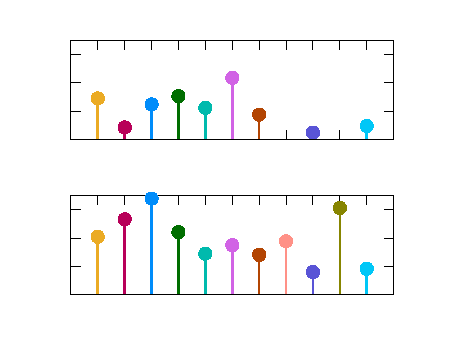
\includegraphics{./figures/parts/appendix/chapters/03/sections/04/csal_location_errors}}%
    \gplfronttext
  \end{picture}%
\endgroup

  \end{subfigure}
  \vspace{1cm}
\caption{\small Μέση τιμή σφάλματος προσανατολισμού ορθών λύσεων (αριστερά) και
         θέσης (δεξιά) ανά στάση στο περιβάλλον CSAL}
\label{fig:appendix:03_04:csal_orientation_position_errors}
\end{figure}
